\documentclass[a4paper]{article}

\usepackage[english]{babel}
%\usepackage[utf8x]{inputenc}
\usepackage{amsmath}
\usepackage{graphicx}
\usepackage[colorinlistoftodos]{todonotes}
\usepackage{natbib}
\usepackage{soul}%allows highlighting \hl{text}
\usepackage{listings}
\usepackage{hyperref}
\title{Representing Algorithms' Performance}
\author{Kevin Sim and Emma Hart and Ben Paechter}


\begin{document}
\maketitle

\begin{abstract}
This review conducts a \hl{not really brief and a bit self indulgent} summary of the literatue relating to how best to represent problem instances and algorithm performance with a view towards being able to perform machine learning on this data. The aim of the review is to check what sort of techniques a new meta-heuristics framework and repository should cover, including existing and potentially future techniques. 

\end{abstract}

%This is shown in Figure \ref{img:Paechter}

%\begin{figure}
%\centering
%\includegraphics[width=1.0\textwidth]{img/Paechter2014}
%\caption{\label{img:Paechter} Taken from \cite{?} the Figure shows ...}
%\end{figure} 



Before describing the literature relating to algorithm performance a brief review of the various techniques used to define problem instances is conducted.

\section {Problem Instance Definitions}

There are many different data sets available to researchers studying optimisation problems. See \cite{floudas2013handbook} for many examples. Although some attempts to create a centralised resource have been relatively successful, many different formats are in use and many publications exist that cite no longer accessible web based resources.

Examining some of the data sets available in commonly used repositories for optimisation and machine learning, such as the OR-Llibrary \citep{OR1990} and the UCI Machine learning Repository, shows that the most common method for storing and distributing problem instances is as individual text files.
However individual data sets, even those created for the same problems, are typically formatted by the creators using bespoke schemas.
Although these are usually relatively straightforward, the variety of different formats leads to a lack of interoperability and an unnecessary overhead in terms of the requirement to develop parsers for each different format.

It seems logical that any repository of metaheuristics and their components should also include formal descriptions (signatures) for common problems, and provide standards for formatting and distributing problem instances. 

Although the scope of this review is to investigate representations for problem \emph{instances} there is often ambiguity and redundancy in the description of the problems for which those instances are designed. 
A complete problem description should include not only a description of the entities involved but also the constraints imposed on, and between, those entities and a description of how to represent and evaluate solutions.

As an example, for a particular instance of a Job Shop Scheduling Problem, a single solution can differ in quality depending on the objective fitness function used to evaluate it (e.g makespan or total weighted tardiness).
Also in the literature instances designed for one problem are frequently used for a variation of that problem: e.g. A vehicle routing problem instance designed for the CVRPTW can be used as an instance for the CVRP or the VRPTW by disregarding the parts of the data irrelevant for the less constrained version of the problem . 

Tools such as heuristic lab (HL) already implement custom designed parsers to convert from the many variations of representations used for problem instances to an internal representation for that domain. 
As an example HL allows users to import VRP benchmark instances in TSPLib format (CVRP), Solomon format (CVRPTW), ORLib format (CVRP) and Cordeau format (Multi depot CVRP / CVRPTW).
This allows users to tackle problems without having to concern themselves with the task of converting different formats. This opens up the possibility of using such tools to export differently formatted benchmark data sets using an already well defined internal representation.

While simple formats such as txt and csv are an efficient means of storing and distributing instance data the number of different bespoke formats make them difficult to interpret, especially as the number of entities and constraints in the problem increases.
For describing the actual problem (Structure, Constraints, Fitness Metrics etc), data definition languages  seem a more appropriate tool that can be used by researchers to re-create problem models in a choice of high level languages. Individual instances can then be represented using recognised standards such as XML, REST or similar and parsed using standard tools that are readily available for most high level programming languages.

%Open source protocols such as XSD, REST, AJAX, XML, UML, OpenMath etc etc could be used to define problems and recreate models and to represent existing and future problem instance data sets.
%
%Attempts to formally define problem formats include the DIMACS format for CNF and SAT problems  \cite{Gu96algorithmsfor} Miller's integer programming formulation of the travelling salesmen problem Miller1960

Recently we have proposed an object oriented model that allows for a number of different rich vehicle routing problems to be described \cite{EuroGEN2015}.
The model is illustrated in the paper using the Unified Modelling Language (UML) and more formally as an XML Schema Definition (XSD) to facilitate recreation of the model on different platforms . 
The problem instances that were generated (4800 in total) are available for download in XML format, are human readable and can be easily be imported by the end-user using any available XML parser implemented for their programming language of choice.

Note that in addition to the {\em attributes} that describe problem (e.g. number and size of items in binpacking, city locations for TSP) there are additional elements that should be included in any definition:

Firstly the constraints of the problem need to be known.  Secondly an objective function for the problem \emph{solution} needs to be defined, so that what constitutes a good solution is known.  The third item that needs to be defined is the objective function for the performance of the  \emph{algorithm}. 


Note that this third specification is often missing from problem instance sets, and is most often defined as part of the experimental design for a particular study. This makes real comparison of algorithms difficult and has the danger that authors might define an algorithm performance objective function that makes their own algorithm look good. This isn't particularly good science and in practice can lead to algorithms that seem good in theory, but don't actually deliver what the user is looking for. Although it is useful to know the algorithm objective functions on which a particular algorithm does well  (or badly), it is better science, and practically more useful, to define in advance what the user is looking for, and then measure all of our algorithms against that benchmark. It is perfectly reasonable of course to define a number of different algorithm objective functions for a particular set of constraints and solution objective functions. Having a different algorithm objective function means that (by the definition of the problem instance given by \cite{Paechter2014}) you have a different problem instance and different algorithms might be the best at solving that instance.  This is discussed further below in relation to algorithm performance.


\section{Algorithm Performance}
What do we mean by algorithm performance and how can we represent experimental results in order to facilitate the comparison of different algorithms' performance and aid knowledge discovery?

The ability to predict the performance of an algorithm is encapsulated in the description of the Algorithm Selection Problem given by \cite{Rice1976} and visualised in Figure \ref{rice}.

\begin{figure}[h!]
\centering
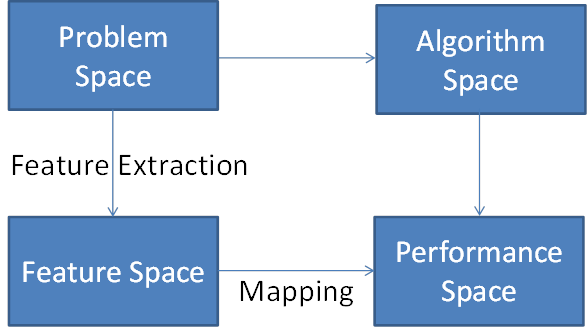
\includegraphics[width=0.5\textwidth]{img/rice}
\caption{\label{rice} The problem of selecting the best algorithm for a problem is described by \cite{Rice1976} as involving finding a mapping between the performance space and a suitable feature space that allows a correlation between performance and problem features for the given algorithm and problem space. 
}
\end{figure} 

Given an algorithm space (set of algorithms), a problem space (set of problem instances) and a suitable solution fitness metric then the set of results returned by the algorithm portfolio is what Rice refers to as the the performance space. This performance space, suggests Rice, can be mapped to the algorithm space by finding a suitable function (machine learning technique) to transpose the instance space into a suitable feature space that allows a correlation to be made between the characteristics of an instance and the quality of the solution returned by an algorithm.
In order to move towards the goal of automatic algorithm selection practitioners must present results from their studies (performance space) in a manner that supports the use of machine learning techniques. The ability to extrapolate a mapping from feature space to performance space relies on researchers providing comprehensive data from their studies.

There are many criteria that can be used to measure algorithm performance from the perspective of the end user. These include : 

\begin{itemize}
\item Run time (Big-O notation)
\item Solution quality and robustness (average performance and standard deviation)
\item Speed of convergence (solution trajectory)
\item Is mine better than yours (statistical tests)
\end{itemize}

The approaches reviewed here that have been used to compare algorithms' performance concentrate specifically  on (1) the quality (or lack of it) of the solutions returned, after a fixed number of evaluations, for a set of problem instances relative to some known theoretical optimal or derived lower bound and (2) the quality of the solutions returned by a \emph{set} of algorithms relative to each other.
The first method allows an algorithm footprint to be defined for a particular instance space, measured using a specific objective fitness measurement.
The second method allows for a direct comparison of the performance spaces produced by different algorithms .  

Clearly the following need to be unambiguously defined. 

\begin{itemize}
\item The problem domain(s) used
\item The set(s) of problem instances used from each domain
\item The objective function(s) used for each domain
\end{itemize}

Experimental results published in the literature are most often insufficient to allow the use of machine learning techniques to derive useful information about an algorithm's performance.
Current practices where researchers present a summary of their results (e.g. mean and standard deviation), often using highly subjective interpretations that back up their own hypothesises, do not aid the process of scientific discovery.
Allowing researchers access to a repository where they can present comprehensive results from their experiments allowing comparison to the approaches of others can only increase the quality of the scientific research being undertaken by the community.

%Importantly, if only the quality of the final solutions is considered then the run time or more importantly the number of fitness evaluations should be fixed and within acceptable run times for the intended problem domain. If speed of convergence It should be noted that none of these metrics are infallible as algorithm designers could use techniques such as regression to estimate fitness calculations.
%
%~

The following practices would facilitate knowledge discovery and aid comparison of algorithms in terms of different performance metrics .

\begin{itemize}
\item Benchmark problem data sets should be clearly defined including a description of any solution fitness metrics and problem constraints.
\item Problem instances should be sufficiently diverse, in terms of the feature space and problem complexity, from the perspective of the algorithms being compared.
\item Solution quality should be reported for each instance and metric.
\item The solution trajectory (results every $n$ evaluations) should form part of the data.
\item The solution genotype (including a suitably complete description) could be included with results for completeness.
\end{itemize}

%The repository should allow researchers to easily define the intended problem domain and present their solutions whether they are for well researched benchmarks data sets or for bespoke real world applications. Having a standardised method of describing problems and a repository of applicable algorithms would potentially facilitate this.
%The ability to compare algorithms designed to operate on problems with multi or many objective fitness functions also needs to be considered but is out of the scope of this review.
%
%The remainder of this section describes methods for comparing the performance of different algorithms and touches on methods for generating suitable problem data sets. 
%
%\subsection*{Algorithm Performance}
%\label{sec:algComp}


Although the NFL theorem implies that all algorithms have identical mean performance when measured over \emph{all} problems it has been noted \citep{Igel2005} that this is unlikely to be relevant in practice when we limit our interest to the performance of an algorithm over a finite subset of domain specific problem instances. \cite{SmithMiles2014} question whether the NFL applies to instances of a specific optimisation problem, using only a subset of possible optimisation functions concluding that any given algorithm is likely to have strengths and weaknesses.

\cite{SmithMiles2014} recently proposed a methodology that allows the strengths and weaknesses of different metaheuristic algorithms to be compared.
For a given a set of algorithms and a set of problem instances each algorithm has a {\em footprint} in the space defined in terms of its performance on an instance relative
to the other algorithms in the set. An algorithm is said to be
$\epsilon$-{\em good} if it achieves a result within $\epsilon$ \% of
the best algorithm in the set. Thus, the footprint of an algorithm
defines the region of the instance space in which it is expected to
perform well.


\begin{figure}
\centering
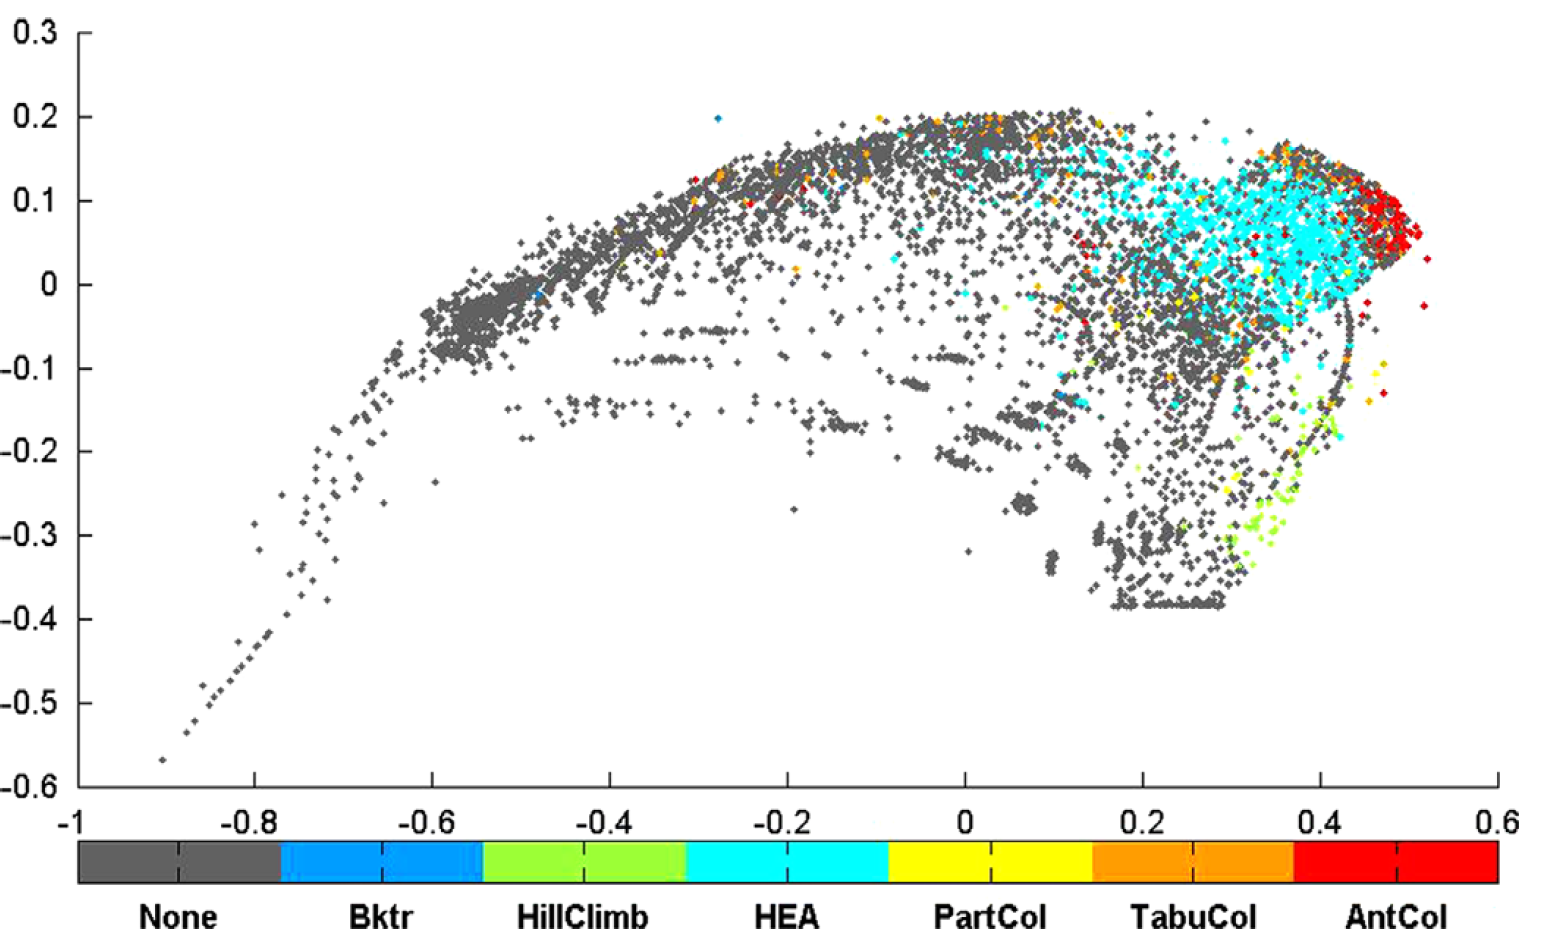
\includegraphics[width=1.0\textwidth]{img/smithBest}
\caption{\label{img:smithBest} Taken from \cite{SmithMiles2014} the plot shows a set of problem instances plotted in a 2-dimensional feature space. Coloured instances indicate that the corresponding algorithm uniquely finds the best found solution}
\end{figure} 

In Figure \ref{img:smithBest} \cite{SmithMiles2014} visualise the performance of a 6 metaheuristic algorithms with respect to the problem characteristics exhibited by each instance.
Each instance is plotted on a 2-dimensional projection of the feature space that is obtained by applying Principal Component Analysis (PCA) to reduce a carefully selected set of problem specific characteristics to the 2 principal eigenvectors.
For each instance where a single algorithm achieves the best found solution, colour coding is used to identify that algorithm. Instances shaded gray are solved equally well by more than 1 algorithm and can be considered as easy for the algorithm portfolio.

This approach allows for a visualisation of relative algorithm performance with respect to a predefined set of characteristics and facilitates understanding and knowledge discovery. However the approach would appear to have limitations as the number of algorithms in the ensemble increases and furthermore relies on being able to manually specify a suitable feature space, a task investigated for a number of CO problem domains in \cite{Smith-Miles219}.

In contrast,recent research in the domains of Bin Packing and Job Shop Scheduling \citep{Sim2013ecj,Sim2015GECCO,Hart2015underReview} has exploited the hypothesis that no heuristic performs best across the complete instance space, to generate ensembles of heuristics that cooperate to improve collective performance across large problem sets. To use terminology from the machine learning literature the method can be described as a ``mixture of experts'' methodology where an ensemble of heuristics is used to solve a set of instances. A generative Hyper-heuristic framework named NELLI is trained on large sets of problem instances resulting in an ensemble of reusable heuristics that are evaluated on a large unseen test set of similar instances. 
During training, individual heuristics survive only if they manage to find higher quality solutions to a niche set of the complete set of training problem instances. 
Similarly problem instances survive if they are only solved best by a single heuristic. 
The resultant set of heuristics sustained by the system can be described as diverse in terms of their respective performance spaces when compared to the other heuristics in the ensemble on a per instance basis, and the problem instances sustained from the training set can be described as ``hard'' and are suitable for comparing those algorithms' performance.

\begin{figure}
\centering
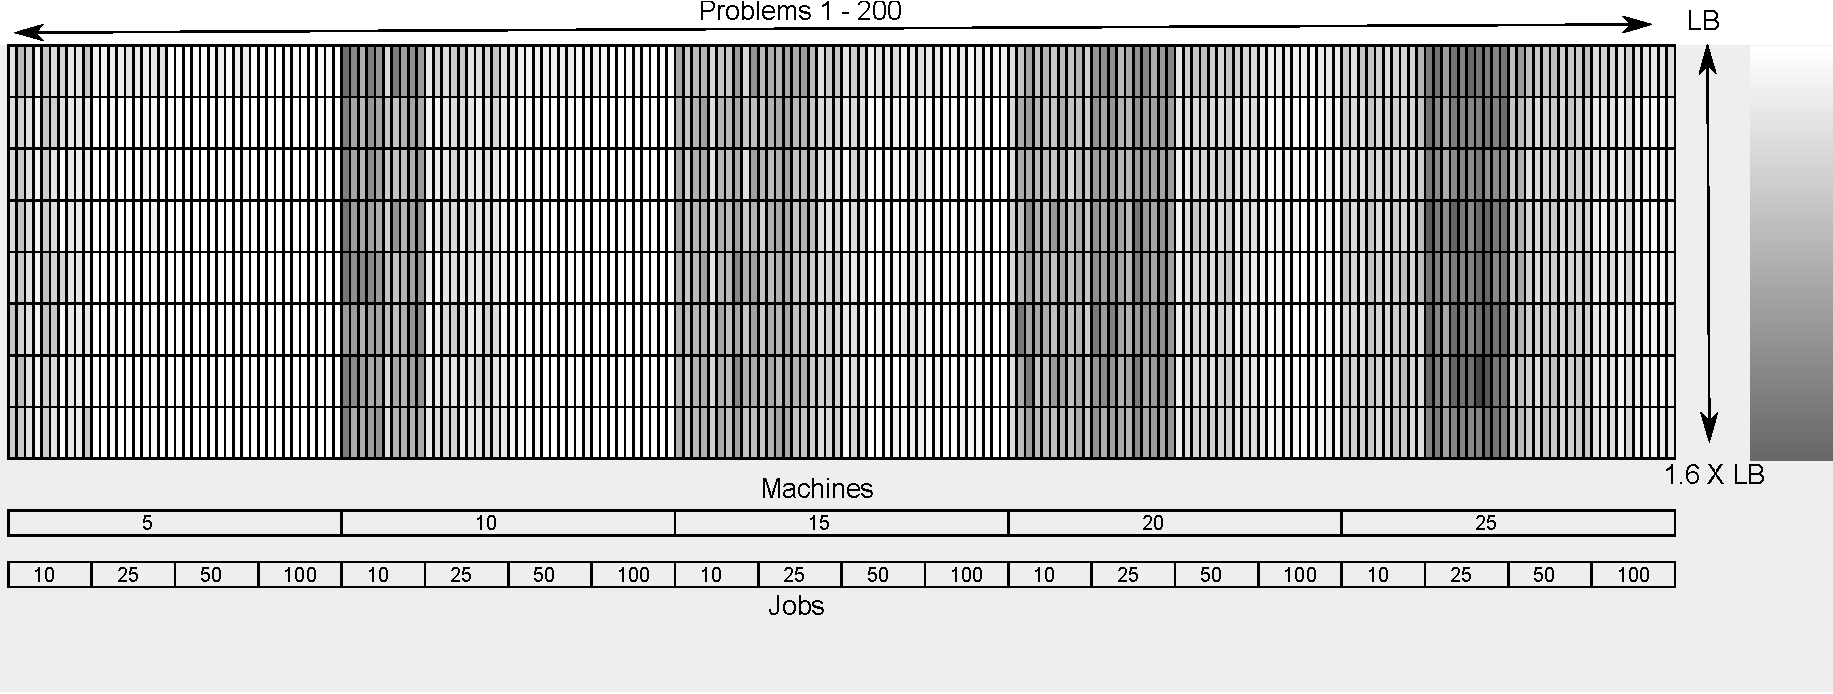
\includegraphics[width=1.0\textwidth]{img/8HProfileBounds}
\caption{\label{img:lb}  An ensemble of 8 heuristics' (rows) performances across 200 problem instances (columns) relative to the theoretical lower bound: ``Lighter" shades indicate a result closer to the theoretical lower bound and ``darker" shades show a solution of around 1.5X the LB}
\end{figure} 

Rather than attempting to reduce the instance space to two dimensions, in \cite{Hart2015underReview} the instance space is visualised as a sequence of cells that are ordered by the parameters used to generate the problem instances. Figure \ref{img:lb} shows the performance of an evolved ensemble of 8 heuristics when used greedily to solve an unseen set of 200 JSSP instances. Each of the 8 rows represents a different  heuristic from the ensemble and each column represents an individual problem instance. Each cell is shaded according to the quality of the solution that the corresponding heuristic achieves on the corresponding problem instance. White (or lighter) cells indicate a solution at (or near to) the theoretical lower bound and the darkest cells indicate a solution quality around 1.5 X the theoretical LB.

It is clear from Figures \ref{img:lb} and \ref{img:smithBest} that certain problem instances are \emph{easy} from the perspective of the set of (meta)heuristics being compared and that others can be deemed as hard. In Figure  \ref{img:smithBest} the hardest problem instances appear to be clustered when visualised in the reduced 2-dimension feature space.
Instances in Figure \ref{img:lb} are simply ordered by the parameters used to generate the problems (number of machines and number of jobs). For the ensemble of 8 heuristics shown instances where the number of machines is equal to the number of jobs appear the hardest and it is those problem instances which show the greatest diversity in terms of heuristic performance and therefore provide a more useful sub-set of the instance space on which to evaluate those heuristics. Obviously for a different set of heuristics the useful sub-set of the instance space may change but it seems likely that many instances generated using a random uniform distribution are trivial for most algorithms and presenting results on these instances is not worthwhile.
However the areas where the performance of a heuristic are less clearly defined. A heuristic that performs well on a particular problem instance that was generated with a certain set of parameters does not necessarily perform well on other instances generated from the same configuration. This indicates that task of describing a suitable feature space for a particular problem domain is not trivial and that there are nuances in the problem structure that are not apparent from this visualisation.

Clearly, in order to assist a comparison between the performance of different algorithms the set of problem instances that they are tested on must be large, diverse and include many challenging instances. If the optimal solution for an instance is trivial to find, as appears to be the case for many of the frequently used benchmark data sets, then those instances provides no insight into performance of an algorithm. 
As an example, using the 3 well known data sets described in \cite{Scholl209} from the 1D Bin Packing Domain, even the simplest of constructive heuristics (first fit descending) achieves optimal solutions for 782 of the 1210 problem instances if solution quality and optimality is defined using the number of bins in the solution.


Problem sets used by academics to evaluate their algorithms are often generated randomly from a uniform distribution. The relationship between algorithm performance and problem structure has been investigated for the Flow Shop Problem domain in \cite{Watson2002}. The authors conclude that there are ``doubts as to whether superior performance on difficult random scheduling problems translates into superior performance on more realistic kinds of scheduling problems''.
Using EC techniques to generate more challenging problem instances has been investigated in  \cite{vanHemert2006,Smith-Miles2010,SmithMiles2015b}. 


\begin{figure}
\centering
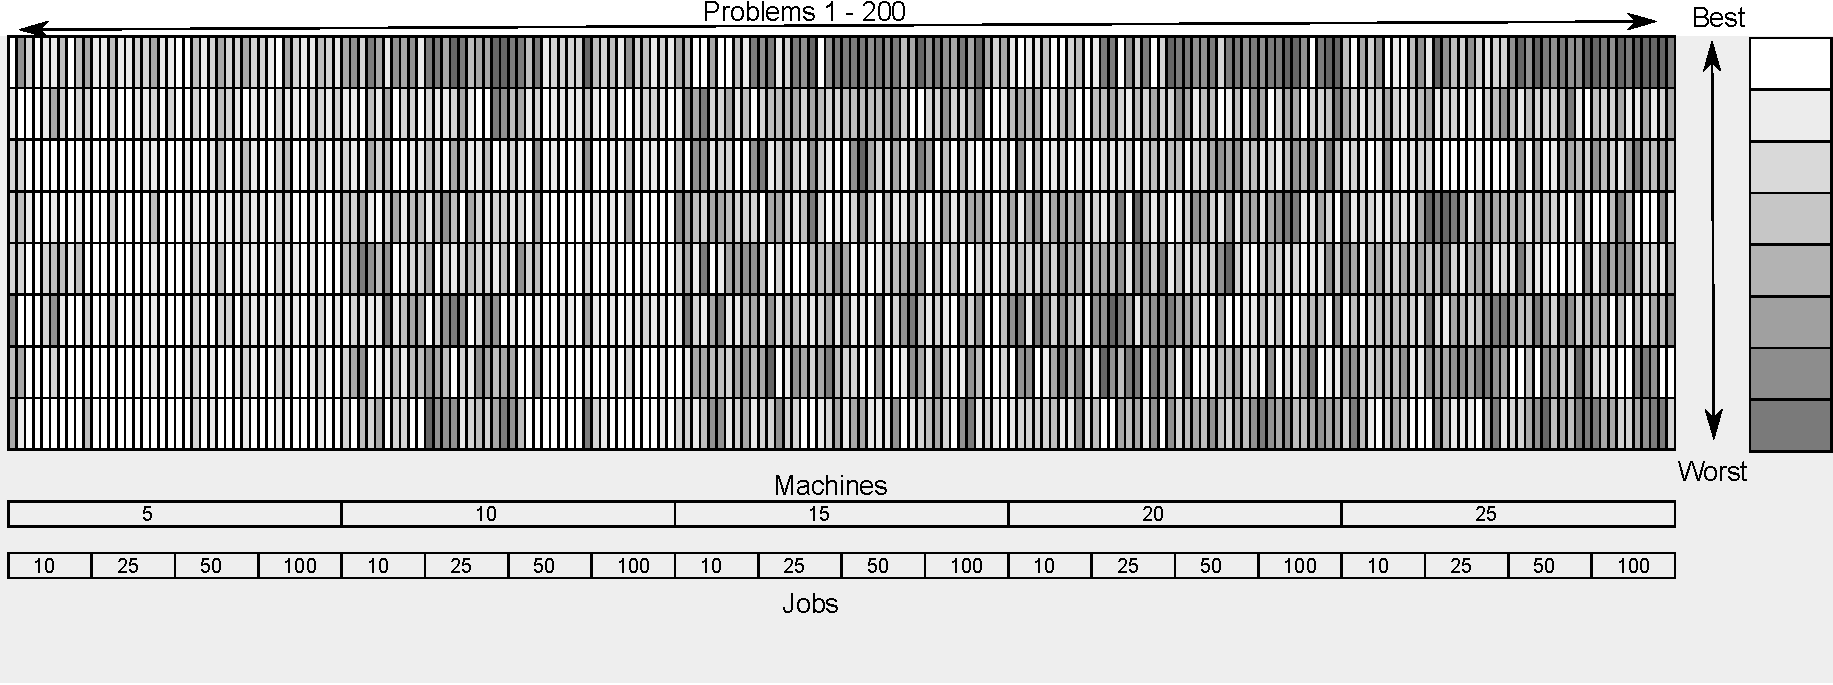
\includegraphics[width=1.0\textwidth]{img/8HProfileRanked}
\caption{\label{img:rank}  An ensemble of 8 heuristics' (rows) performances across 200 problem instances (columns) relative to each other: White cells indicate a result that is best or joint best on that instance. Dark cells indicate relatively poor performance on that instance compared to the best found solution}
\end{figure} 

 In \cite{Hart2015underReview} the system used to generate the ensemble guarantees that there will be differences in the set of solutions produced by each heuristic. However if the quality of each heuristic is measured by averaging results across all test instances then all appear similar and the strengths and weaknesses of individual heuristics is lost. Having access to more comprehensive results would facilitate knowledge discovery in a way that the practice of reporting average or summarised results on small benchmark problem sets excludes. 

For a given set of algorithms $\mathcal{H}$ and a large test set of diverse problem instances $\mathcal{P}$ comparing the footprint (vector of results) of each heuristic in  $|\mathcal{H}|  \times |\mathcal{P}|$ matrix provides a quick and easy method of identifying where methods perform well or where they perform badly.

Figure \ref{img:rank} visualises the same results used to generate Figure \ref{img:lb} but rather than shading a cell based on the quality of the solution relative to a lower bound the cell is shaded based on the ranking of the heuristic on that instance relative to solutions achieved by the other heuristics in the ensemble. 
This allows the relative performance of a set of heuristics to be visualised without the need to define a reduced feature space, or the need to calculate a lower bound. Two heuristics that appear almost identical in terms of their performances when averaged across the complete instance space may actually prove to be diverse when compared on an instance to instance basis.

\section*{Interesting Papers to read}

Hyper-heuristics have been touted as procedures capable of transcending domain barriers but in order to justify these claims both good and bad results need to be presented. \cite{Misir20133335} investigated the level of generality of 14 selection hyper-heuristics applied to three different problem domains (
home care scheduling, nurse rostering and patient admission scheduling). The authors concluded that the performance of individual hyper-heuristics changes significantly under different experimental conditions highlighting the need for larger empirical investigations to back up the claims of generality made by many in the community.

\cite{Blum2003} conduct a review of common metaheuristics in order to outline the structural similarities and differences in the different components and concepts used.
Thir I\&D framework allows metaheuristics to be described in terms of their intensification and diversification mechanisms, which the authors suggest ``largely determine the behaviour of a metaheuristic''. While this approach allows algorithms to be compared in terms of their structural similarities it does not allow knowledge discovery techniques to be used to derive useful information relating to an algorithms' performance.

\subsection{Examples of Problem Libraries}

A good resource with links to some of the many problem libraries in the wild.

 \url{http://www.mat.univie.ac.at/~neum/glopt/test.html\#test_combin}
  
{\bf Can consider how the problems in the following libraries are made available}

\begin{itemize}
\item One of the most persistent is the OR-Library \citep{OR1990} which hosts a collection of data sets for several combinatorial optimization problems. Other resources include the DIMACS satisfiability benchmarks Implementation Challenge a set of instances were chosen to provide the satisfiability benchmarks. These problems can be found at http://dimacs.rutgers.edu/Challenges/index.html.SAT problem 


\item During the second DIMACS Implementation Challenge a set of instances were chosen to provide the satisfiability benchmarks. These problems can be found at http://dimacs.rutgers.edu/Challenges/index.html.

\item A large collection of Traveling Salesman test problems is available at http://www.iwr.uni-heidelberg.de/iwr/comopt/soft/TSPLIB95/TSPLIB.html.

\item A QAP test problem generator with a known optimal solution is available. The Fortran code of this generator can be obtained by sending an e-mail message to coap@math.ufl.edu and in the body of the message put ``send 92006''.

\item There is a large collection, QAPLIB, of electronically available data instances for the Quadratic Assignment Problem. The data (and the updated best known solution) are available at http://www.diku.dk/users/karisch/qaplib/inst.html.


\item During the second DIMACS Implementation Challenge a set of 32 graph instances were chosen to provide benchmarks for the Graph Coloring Problem. These problems can be found at http://dimacs.rutgers.edu/Challenges/index.html.
\end{itemize}





\bibliographystyle{apalike}
\bibliography{representing-algorithms-performance}
\end{document}